% \clearpage
% \phantomsection% 
% \addcontentsline{toc}{chapter}{HALAMAN PERNYATAAN ORISINALITAS}

% \begin{center}
% 	\smallskip
	
% %	\chapter*{\normalsize{Halaman Pernyataan Orisinalitas}}
% 	\large \bfseries \MakeUppercase{Halaman Pernyataan Orisinalitas} \linebreak
	
% 	\normalsize  \normalfont \justify \onehalfspacing{
% 		Saya yang bertanda tangan di bawah ini\\
		
% 		Menyatakan bahwa Tugas Akhir dengan judul : “{\thetitle}” adalah benar karya saya sendiri. Seluruh sumber baik yang dikutip maupun dirujuk dalam penulisan tugas akhir ini telah saya cantumkan secara benar sesuai dengan kaidah penulisan ilmiah.\\
		
% 		Apabila di kemudian hari ditemukan adanya unsur plagiarisme dalam karya ini, maka saya bersedia menerima sanksi sesuai ketentuan yang berlaku di institusi saya.\\
		
% 		Demikian pernyataan ini saya buat dengan sesungguhnya.
% 		}
% 	\vspace{3cm}
	
% 	\centering 
% 	Lampung Selatan, \todayIndo\\
% 	\vspace{2cm}
% 	\theauthor\\
% 	NIM. \printnim
% \end{center}
% \clearpage

% \clearpage
% \phantomsection% 
% \addcontentsline{toc}{chapter}{HALAMAN PERSETUJUAN PUBLIKASI}

% \begin{center}
% 	% \small % Add this line to make the font smaller
% 	\smallskip
	
% 	\normalsize \bfseries \MakeUppercase{
% 		HALAMAN PERNYATAAN PERSETUJUAN PUBLIKASI \\
% 		TUGAS AKHIR UNTUK KEPENTINGAN AKADEMIS
% 	}\linebreak
	
% 	\normalfont \onehalfspacing \justifying % Changed \normalsize to \small
% 	Sebagai civitas akademik Institut Teknologi Sumatera, saya yang bertanda tangan di bawah ini:
	
% 	\flushleft
% 	\setlength{\tabcolsep}{0pt}
% 	\begin{tabular}{l l}
% 		Nama 			&  : \theauthor\\
% 		NIM 			&  : \printnim\\
% 		Program Studi \	&  : Teknik Informatika\\
% 		Fakultas 		&  : Teknologi Industri\\
% 		Jenis Karya 	&  : Tugas Akhir\\
% 	\end{tabular}

% 	\justifying
% 	\noindent demi pengembangan ilmu pengetahuan, menyetujui untuk memberikan kepada Institut Teknologi Sumatera \textbf{Hak Bebas Royalti Noneksklusif \textit{(Non-exclusive Royalty Free Right)}} atas karya ilmiah saya yang berjudul:
	
% 	\centering
% 	\textbf{\thetitle}
	
% 	\justifying
% 	beserta perangkat yang ada (jika diperlukan). Dengan Hak Bebas Royalti Noneksklusif ini Institut Teknologi Sumatera berhak menyimpan, mengalihmedia/formatkan, mengelola dalam bentuk pangkalan data (\textit{database}), merawat, dan memublikasikan tugas akhir saya selama tetap mencantumkan nama saya sebagai penulis/pencipta dan sebagai pemilik Hak Cipta.
	
% 	Demikian pernyataan ini saya buat dengan sebenarnya. \\
	
% 	\centering
% 	Lampung Selatan, \todayIndo\\
% 	\bigskip
% 	Yang menyatakan\\
% 	\vspace{1.5cm}
% 	\theauthor\\
% 	NIM. \printnim\\
	
% \end{center}
% \clearpage


\clearpage

\phantomsection% 
\addcontentsline{toc}{chapter}{HALAMAN PERNYATAAN ORISINALITAS}

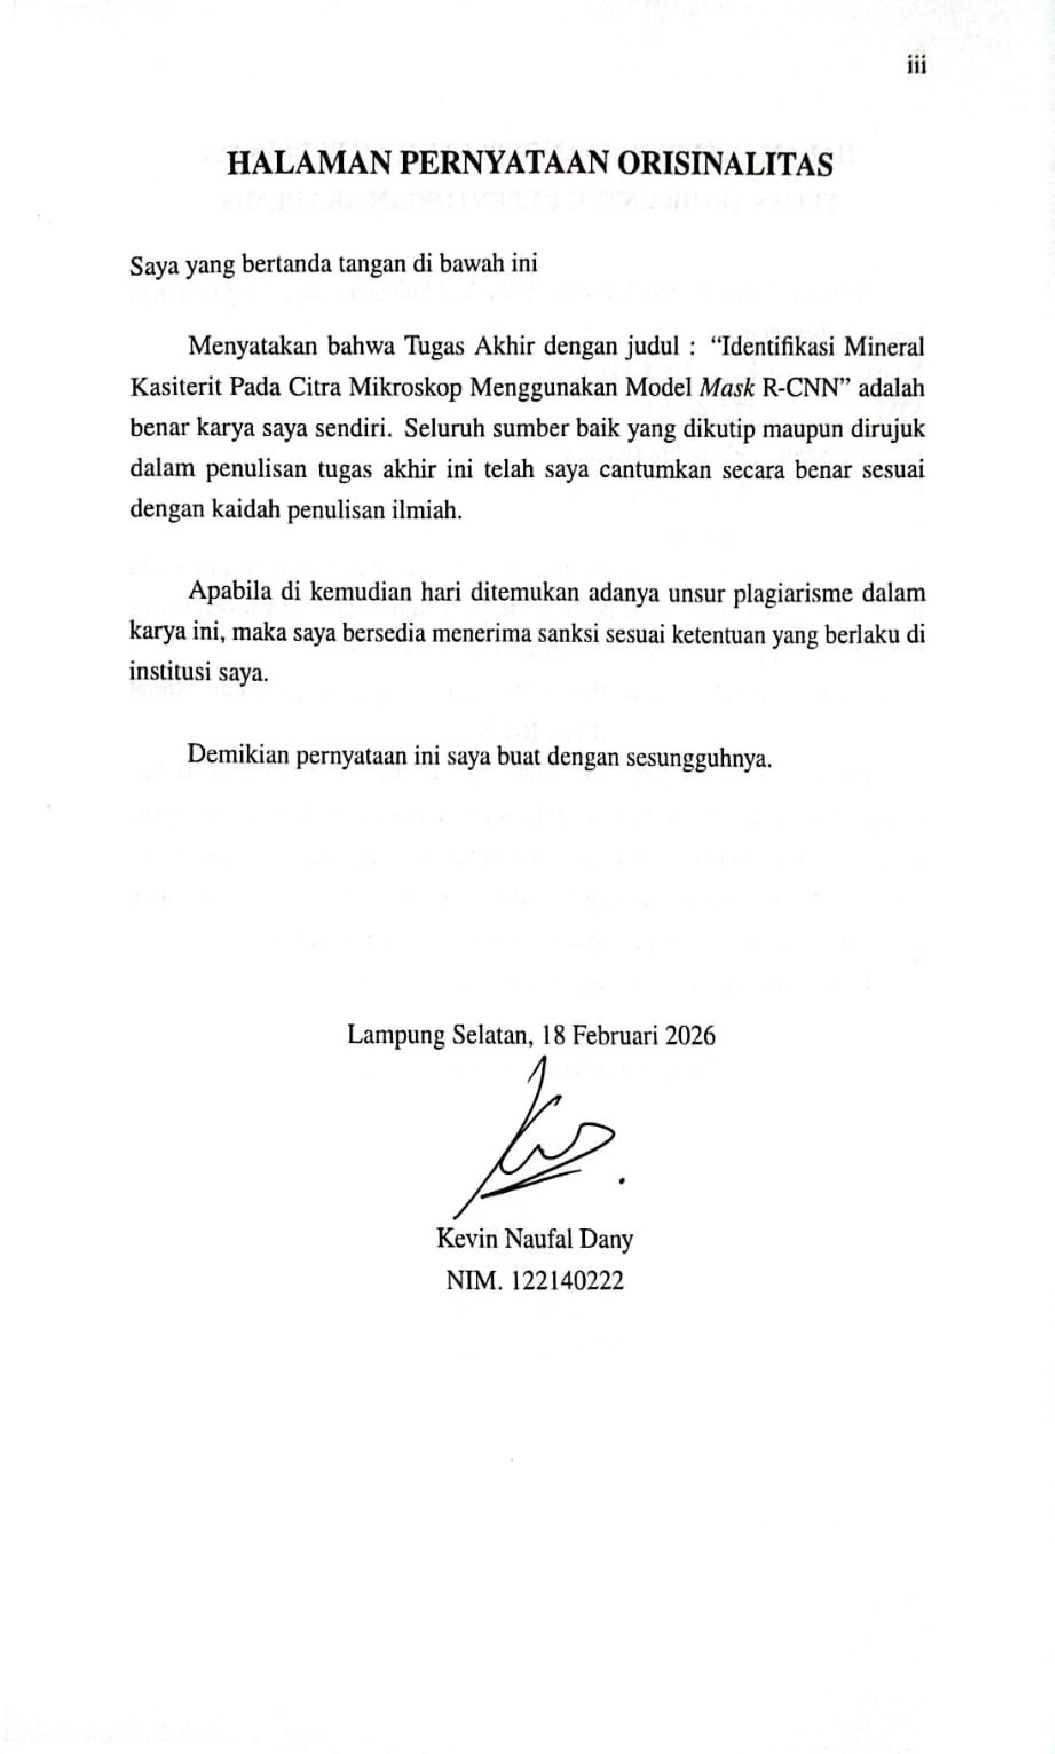
\includepdf[
    pages=1,
    width=\paperwidth,
    height=\paperheight
]{doc/orisinil.pdf}

\clearpage